\thispagestyle{empty}
\begin{center}
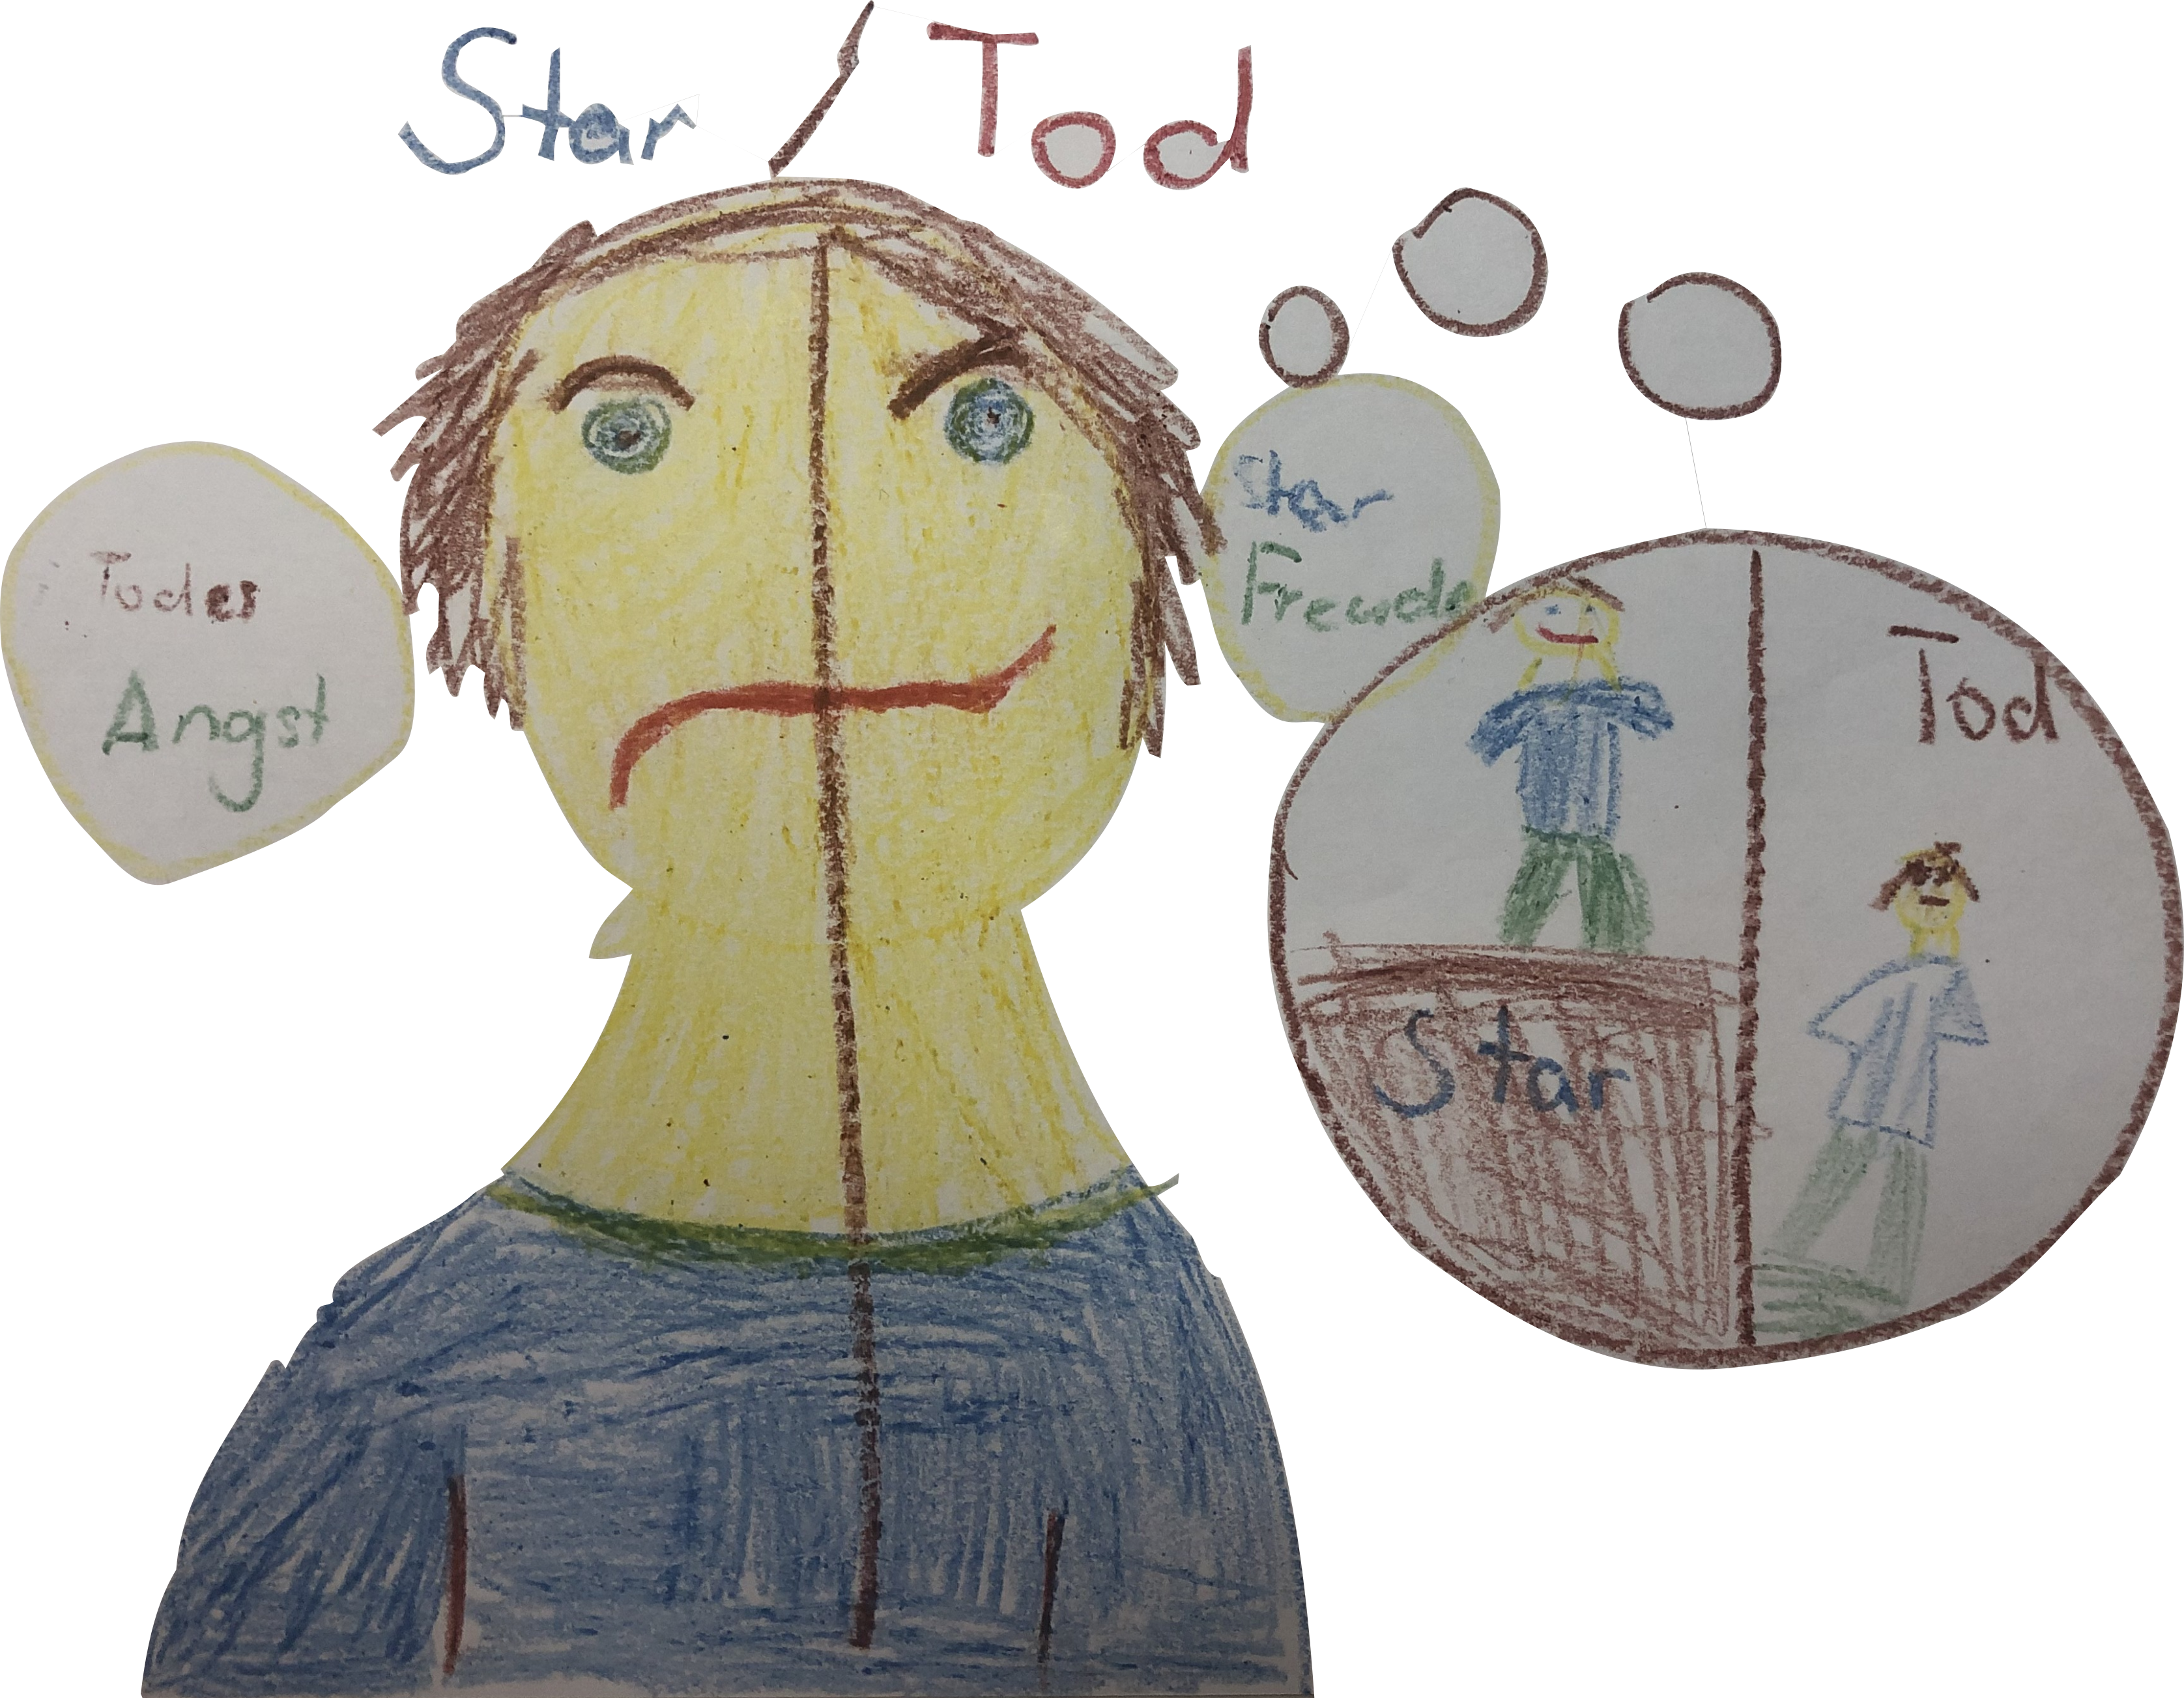
\includegraphics[width=\textwidth]{./bilder/drache.png}
\end{center}
\vspace*{\fill}
{\centering\fontsize{50}{48} \color{farbe}\sffamily{Milly}\par}
\addcontentsline{toc}{chapter}{Milly im Runden Eck}
\newpage
%%%%%%%%%%%%%%%%%%%%%%%%%%%%%%%%%%%%%%%%%%%%%%%%%%%%%%%%%%%%%%%%%%%%%%%%%%%%%%%
\lettrine[lines=3, lhang=.2, loversize=.25, lraise=0.05, findent=0.1em,
nindent=0em]{D}{amen} gab es keine, im \textit{Im Runden Eck}. Das lag nicht an der fehlenden Präsenz weiblicher Kundschaft, über die so viele Kneipen sonst zu klagen haben, sondern an Milly.

Das \textit{Im Runden Eck} war ein echtes Relikt, wobei das kaum jemand merkte, da vielen die Aussenwelt unbekannt war. Gelegenheitsbesucher gab es kaum, man kannte sich oft schon aus der Zeit der Gründung des \textit{Im Runden Eck}. Früher, als das \textit{Im Runden Eck} als Kooperative, der ideologisch einzig mögliche Organsiationsform, bezeichnet, in Wahrheit aber doch Alfi geführt wurde. Er hatte von allen am

Zeiten, als Sozial- und Geisteswisschaffende noch dachten, mit ihren leider meist karrikaturhaft unverstehbaren Veröffentlichungen 

gesellschaftliche Relevanz, gar deren geistige Führerschaft beanspruchen zu können, ach was, zu müssen, klumpten sich an verschiedenen bis dahin nicht durch Relevanz geprägter Quartiere einiger grösserer Städte junge Menschen, die oft im Überschwang drogenkatalysierter erwachender Hormonvielfalt.

Denn seien sie sich versichert, sollte sie sich nicht gerade unbedingt alleine auf einer einsamen, besser noch unendeckten Insel befinden, die keinerlei Bequemlichkeiten moderner Kommunikation kennt, und sie nicht gerade Rekorde im Extrem-Höhlen-Tauchen aufstellen, sei ihnen dringend vom Gebrauch von Vokabeln wie \textit{Dame} abzuraten. Milly hatte seit jeher zu solchen Fragen eine sowohl klare, wie auch ausgesprochen umfangreiche Meinung, deren wichtigste Eigenschaft allerdings war, dass sie mit sonst nur aus der theoretischen Informatik bekannten strikten Notwendigkeit zum Vortrag gebracht wurde. Die von Milly gewählte Form des Vortrags war der Gruppe der Beleidigungen, grobe, zuzurechnen. Da die Rede über Jahrzehnte von einer sehr scharfsinnigen, stets verfeinert worden war, konnten die Skeptiker an Millys Meinung letztendlich nur höchst nichtssagende Gegenargumente wie dass das ja wohl bitteschön etwas übertrieben sei und man doch auch bitteschön die Verhältnismässigkeit im Auge behalten solle. Aber mit Bitten war da nichts zu machen. Zumal das Publikum der Arena dieser setse so ungleichen Kämpfe, der Kneipe \textit{Im Runden Eck} allesamt zwar spätestens von Milly von aller Heräsie befreit wurden, aber sich auch sonst in einem Milieu bewegten, dass Konzepten wie Damenhaftigkeit mit einer Spektrum von Reaktionen reagierte, die mit Naserümpfen beginnt und mit Nasepflücken endet.


seit einiger Zeit 55


Nur für den genialen Hutmacher 

langer spanischer name

aus der Nähe von Mannheim war so eine Impertinenz folgenlos. Aber das ist eine ganz andere Geschichte.


\hfill \pgfornament[color=farbe,height=.5cm]{3}

\newpage
 

